\documentclass[t]{beamer}
\usepackage{CJKutf8}
\usepackage{amsfonts}
    \usepackage{amsmath}
    \usepackage{amssymb}
    \usepackage{amsthm}
    \usepackage{enumerate}
    \usepackage{graphicx}
    \usepackage{layout}
    \usepackage{mathrsfs}
    \usepackage{fancyhdr}
    \usepackage{subfigure}
    \usepackage{tcolorbox}
    \usepackage{tikz-cd}
    \usepackage{color}
    \usepackage{pifont}
    \usepackage{verbatim}
    \usepackage{mathtools}
    \usepackage{float}
    \usepackage{bm}
    \usetheme{AnnArbor}
% \usetheme{Antibes}
\usecolortheme{beaver}
\usepackage{listings}

% 设置JSON样式
\lstdefinestyle{json}{
    basicstyle=\tiny\ttfamily,
    columns=fullflexible,
    showstringspaces=false,
    commentstyle=\color{gray},
    keywordstyle=\color{blue},
    stringstyle=\color{red},
    breaklines=true,
    frame=single,
    captionpos=b,
    aboveskip=10pt,
    belowskip=10pt
}

\lstset{
    language=Python, % 设置代码块语言为Python
    breaklines=true, % 自动换行
    basicstyle=\small\ttfamily, % 设置基本字体样式
    keywordstyle=\bfseries\color{blue}, % 设置关键字样式
    commentstyle=\itshape\color{gray}, % 设置注释样式
    showstringspaces=false, % 不显示字符串中的空格
    frame=single, % 设置代码块边框样式
    numbers=left, % 行号显示在左侧
    numberstyle=\tiny\color{gray}, % 设置行号样式
    stepnumber=1, % 设置行号间隔
    tabsize=4 % 设置制表符宽度
}


% 设置shell样式
\lstdefinestyle{shell}{
    language=bash,
    basicstyle=\tiny\ttfamily,
    columns=fullflexible,
    showstringspaces=false,
    commentstyle=\color{gray},
    keywordstyle=\color{blue},
    stringstyle=\color{red},
    breaklines=true,
    frame=single,
    captionpos=b,
    aboveskip=10pt,
    belowskip=10pt
}

\usepackage{subfigure}

% 添加网址的命令
\usepackage{hyperref}
% 这是一个带链接文本的示例:\href{https://www.example.com}{点击这里访问网站}
% 普通的示例:\url{https://www.example.com}
% 表格
\usepackage{booktabs}
\usepackage{multirow}

% \setbeamertemplate{navigation symbols}{}

\usepackage{textpos}

\newcommand{\dif}{\mathrm{d}}
\newtheorem{thm}{{定理}}

% some common command
\newcommand{\mm}[1]{$ #1$\newline}
% \newcommand{\tuichu}{\Rightarrow}
% \newcommand{\li}[1]{\newline#1}



\newcommand{\analysis}[2]{\forall \mathcal{E}{#1},\exists \delta {#2},s.t.}
\newcommand{\denyanalysis}[2]{\exists \mathcal{E}{#1},\forall \delta {#2},s.t.}
\newcommand{\yield}{\Rightarrow }
\newcommand{\jj}{\newline}
\newcommand{\ff}[1]{$ #1$}   % math environment + newline
\newcommand{\fgn}[1]{\begin{equation}#1\end{equation}  }
\newcommand{\fg}[1]{$$ #1$$}   % math environment + newline 
\newcommand{\pf}{$proof.$\newline}
\newcommand{\ee}{\newline\ff{\Box}\newline}
\newcommand{\fenshi}[2]{\ff{\frac{#1}{#2}}}
\newcommand{\shenlue}{\vdots\jj}
\newcommand{\abs}[1]{{\left \lvert #1 \right\rvert}}
\newcommand{\loge}[1]{In ({#1})}
\newcommand{\logical}[2]{log_{#2}^{#1}}
\newcommand{\summary}[3]{$\sum_{{#1}={#2}}^{#3}  $}
\newcommand{\denjia}[2]{{#1}\Leftrightarrow {#2}}
\newcommand{\jihe}[3]{ {#1}  = \{ {#2} \mid {#3} \} }
\newcommand{\ve}[2]{\left\langle {#1},{#2}\right \rangle}
\newcommand{\dakuohao}[2]{\begin{array}{rcl}{#1}\end{array} \} \Rightarrow{#2}}
\newcommand{\sxb}[3]{#1^{#2}_{#3}}
\newcommand{\sss}[2]{#1^{#2}}
\newcommand{\xxx}[2]{#1_{#2}}
\newcommand{\bri}[1]{\uppercase\expandafter{\romannumeral#1}}
\newcommand{\ri}[1]{\romannumeral#1} 
\newcommand{\polynomial}[8]{#1_{#2}#6^{#7}+#1_{#3}#6^{#8}+...+#1_{#4}#6+#1_{#5} }
\newcommand{\newd}[4]{f[{#1}_{#2},{#4},{#1}_{#3}]}
\newcommand{\lb}[2]{\begin{align*}\begin{split}{#1}\{ {#2}\end{split}\end{align*}}
\newcommand{\tab}[1]{\begin{array}{ll} {#1}\end{array}}


% 向量乘积
\newcommand{\avg}[1]{\left\langle #1 \right\rangle}
% 偏微分方程
\newcommand{\difFrac}[2]{\frac{\dif #1}{\dif #2}}
\newcommand{\pdfrac}[2]{\frac{\partial{#1}}{\partial{#2}}}
% 不同章节
\newcommand{\one}[1]{\section{#1}}
\newcommand{\two}[1]{\subsection{#1}}
\newcommand{\three}[1]{\subsubsection{#1}}
\newcommand{\aone}[1]{\section*{#1}}
\newcommand{\atwo}[1]{\subsection*{#1}}
\newcommand{\athree}[1]{\subsubsection*{#1}}
% 大括号,左右都有
\newcommand{\lbra}[1]{\left\{  {\begin{matrix} #1 \end{matrix}}\right. } 
% 样式 括号前缀 + 括号 
\newcommand{\lbras}[2]{{#1}\left\{ {  {\begin{matrix} #2 \end{matrix}}}\right. } 
\newcommand{\rbra}[1]{ \left.  {\begin{matrix} #1 \end{matrix}} \right\}  } 
% 模长
\newcommand{\distance}[1]{\parallel #1\parallel }
% 等价
\newcommand{\equ}{\Longleftrightarrow }
% 共轭
\newcommand{\cja}[1]{\overline{#1}}
% 两个矩阵,上面是 方框[] 下面是线条| 中间是 无
\newcommand{\mtx}[1]{\begin{matrix}#1\end{matrix} }
\newcommand{\bmtx}[1]{\begin{bmatrix}#1\end{bmatrix} }
\newcommand{\vmtx}[1]{\begin{vmatrix}#1\end{vmatrix} }
% \newcommand{\table}[1]{\begin{array}[lr]{ccc} #1 \end{array}}

%输入普通字符
\newcommand{\ww}[1]{\text{#1}}

% 所有内容 直接头文件搞定
\newcommand{\everything}[1]{\begin{document}\begin{CJK*}{UTF8}{gkai}#1\end{CJK*}\end{document}}


% 存放代码(失败了)
\newcommand{\cccode}[1]{\begin{lstlisting}#1\end{lstlisting}}

% 改变特定行序列
\newcommand{\ttt}{\subsection{}}

% 嵌套序号
\newcommand{\eee}[1]{\begin{enumerate}#1\end{enumerate}}


% 模板里面的一些宏
\newcommand{\pdfFrac}[2]{\frac{\partial #1}{\partial #2}}
\newcommand{\OFL}{\mathrm{OFL}}
\newcommand{\UFL}{\mathrm{UFL}}
\newcommand{\fl}{\mathrm{fl}}
\newcommand{\op}{\odot}
\newcommand{\Eabs}{E_{\mathrm{abs}}}
\newcommand{\Erel}{E_{\mathrm{rel}}}
% 变化颜色
\newcommand{\red}{\textcolor{red}}
\newcommand{\blue}{\textcolor{blue}}
% 注释代码
% \newcommand{\undef}[1]{\iffalse #1 \fi}

% 流程图需要用到的宏包
\usepackage{palatino}
\usepackage{tikz}
\usetikzlibrary{shapes.geometric, arrows}
\tikzstyle{startstop} = [rectangle, rounded corners, minimum width = 2cm, minimum height=1cm,text centered, draw = black, fill = red!40]
\tikzstyle{io} = [trapezium, trapezium left angle=70, trapezium right angle=110, minimum width=2cm, minimum height=1cm, text centered, draw=black, fill = blue!40]
\tikzstyle{process} = [rectangle, minimum width=3cm, minimum height=1cm, text centered, draw=black, fill = yellow!50]
\tikzstyle{decision} = [diamond, aspect = 3, text centered, draw=black, fill = green!30]
% 箭头形式
\tikzstyle{arrow} = [->,>=stealth]
% 4个非常重要 的新命令
\newcommand{\start}[2]{    \node (start) [startstop]{#1};\node (in1) [io, below of = start]{#2};\lin{start}{in1}{}}
\newcommand{\stopp}[3]{\node (out1) [io, below of= #1]{#2};\node (stop) [startstop, below of=out1]{#3};\lin{out1}{stop}{} }
\newcommand{\pro}[6]{    \node (#3) [process, #2 of=#1,xshift=#4 cm]{#5};}
\newpage
\newcommand{\lin}[3]{\draw [arrow] (#1) --node [above] {#3} (#2);}


\begin{document}
\begin{CJK*}{UTF8}{gkai}
% 一般第一页显示PPT标题以及作者信息

% \BackgroundPic{./Screenshot from 2022-04-20 16-31-08.png}

% 增加学校 前面
\addtobeamertemplate{title page}{}{
	\begin{tikzpicture}[remember picture,overlay]
		% \node[yshift=85pt,xshift=50pt]{\includegraphics[height=2cm]{Screenshot from 2022-04-20 16-51-21.png}};
\end{tikzpicture}
}
	% \title{时间序列数据集}
	\title{组会汇报}
	\subtitle {} %不需要
	\author{
		陈钶杰\, \\
		专业:计算数学\,
	} % 显示作者
	% \institute {学院:数学科学学院} % 设置学院机构	
	\date{\today}  % 显示日期
\titlepage

% 设置目录
\begin{frame}{目录}
\frametitle{目录}	
\tableofcontents  % 显示目录
\end{frame}


\section{代码调试}

\begin{frame}
    \frametitle{序列分类模型与自然语言模型对比实验}
    \eee{
        \item 将50支股票分别随机选取6支进行对比实验并进行可视化
        \item 两种模型均是将50组数据合并在一起进行训练的,然后在相应的测试集上进行对比预测结果。
    }
\end{frame}
\subsection{进行序列分类任务,并计算预测误差}

\begin{frame}
    \frametitle{如何进行序列分类任务?}
    \begin{itemize}
        \item 序列分类任务的工作是将文本序列归类到预设类型中,如新闻分类、情感分类等,就属于这类任务。但是我们当前的输入也是一串数据而不是一句话,我选择了图像分类问题的基础模型。\\
        将原本的输入输出\\
        input:1,3,4,10,3,9,3,5,11,6,8,9,3,2,5,6\\
        output:4\\
        以图像的形式该写成:\\
        input:
        \ff{
            \bmtx{
            1 & 3 & 4 & 10 \\
            3 & 9 & 3 & 5  \\
            11 & 6 & 8 & 9 \\
            3 & 2 & 5 & 6
        }}(实际输入的时候会进行归一化)\\
        output: 4(表示类别4)
    \end{itemize}
\end{frame}

\begin{frame}
    \frametitle{如何进行序列分类任务?}
    \begin{itemize}
        \item 但是在处理过程中发现一个的问题,选取的batch\_size = 64,而我们的相邻序列之间的相似度很高,如果不打乱顺序的话会导致每一个batch\_size中的特征趋于统一,导致训练结果变差。\\
        因此事先会将所以训练集进行打乱处理,但是这样处理也会导致每次训练的结果差异变大。
        \item 还有一个问题是图像分类的时候不同图像间的特征是非常明显的,比如数字识别,但是我们这个任务就像是识别一堆主观上来说没有明显特征区分度的图像,不知道是否会导致结果不精确?
    \end{itemize}
\end{frame}


\begin{frame}
    
    \begin{table}[ht]
        \centering
        \caption{准确率结果}
        \large
        \label{tab:example}
        \begin{tabular}{|c|l|r|c|c|c|}
        \hline
        & chatglm & Transformer \\
        \hline
        样例1 & 0.1432 & \red{0.1537} \\
        \hline
        样例2 & \red{0.1721} &0.1060  \\
        \hline
        样例7 & 0.1701 & \red{0.2103} \\
        \hline
        样例8 & 0.1210 & \red{0.1410} \\
        \hline
        样例25 & \red{0.1224} & 0.1064 \\
        \hline
        样例42 & 0.1245 & \red{0.1262} \\
        \hline
    \end{tabular}
        \end{table}
            

\end{frame}

\subsection{预测结果可视化}

\begin{frame}
    \frametitle{\tiny 使用多个时间序列模型进行训练}    
    \begin{figure}[ht]
        \centering
        \subfigure[chatglm测试结果]{
            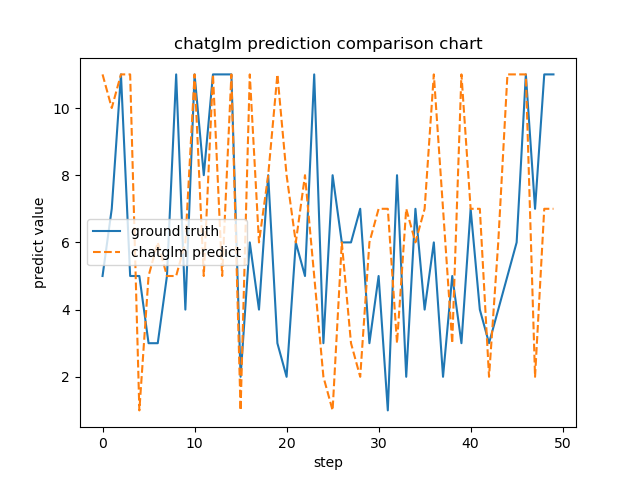
\includegraphics[width=0.45\textwidth]{png/42.png}
        }
        \hfill
        \subfigure[tranformer测试结果]{
            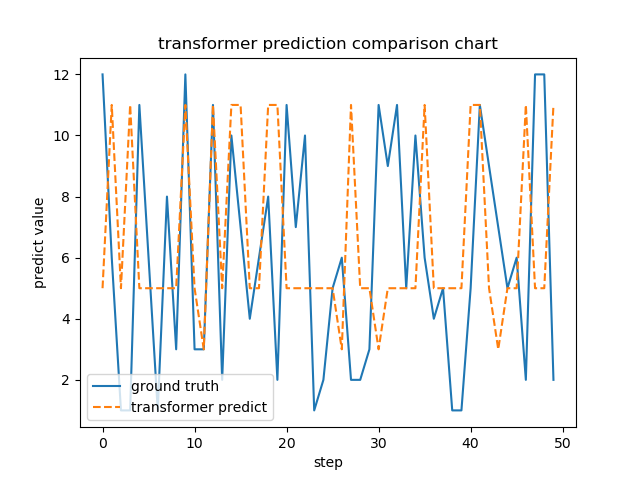
\includegraphics[width=0.45\textwidth]{png/data.png}            
        }
    \end{figure}
\end{frame}


\begin{frame}
	\frametitle{}
	\begin{itemize}
        \item 经过模型测试,两种模型的准确率差不多。
        \item tranformer模型的结果稍稍比chatglm效果好一点,但是不如chatglm模型稳定。
        % \item 总的来说这两种模型来泛化
	\end{itemize}
\end{frame}




% \subsection{下一步的计划}
% \begin{frame}
% 	\frametitle{下一步计划及相关问题}	
% 	\begin{itemize}
%         % \item 使用auto-cot,对比当前的结果
%         % \item 能否将RevIN 增加中间步骤提高结果的精确性。        
%         % \item 提取模型中的注意力权重,查看模型对于输入信息的处理细节
%         % \eee{
%         %     \item 如何解决经过规范化以后数值比较接近的问题?
%         % }
% 	\end{itemize}
% \end{frame}

% 结束语
\section{}
\begin{frame}
	\frametitle{}
	\begin{center}
		\Huge{谢谢老师和同学们的聆听!}
	\end{center}
\end{frame}

\end{CJK*}
\end{document}
